\section{Applicazioni lineari}
\subsection{Definizione: applicazione lineare (trasformazione lineare o homomorfism of vector space)}
Un'applicazione lineare è un'applicazione $T:V\rightarrow W$ di spazi vettoriali su $K$ tale che $\forall v,v_1,v_2\in V$, $\forall\lambda\in K$ si ha:
\begin{enumerate}
	\item $T(v_1+v_2)=T(v_1)+T(v_2)$ ($T$ è additiva)
	\item $T(\lambda\cdot v)=\lambda\cdot T(v)$ ($T$ è omogenea)
\end{enumerate}
(additiva+omogenea = è lineare).
\\In altre parole $T$ conserva le operazioni di spazio vettoriale.

\subsection{Proposizione}
Punti $1+2\Leftrightarrow 3:\; \forall\lambda\mu\in K,\forall v_1,v_2\in V$
\[T(\lambda v_1+\mu v_2)=\lambda T(v_1)+\mu T(v_2)\]
$T$ manda combinazioni lineari in combinazioni lineari (con gli stessi scalari) dei trasformati.

\subsection{Definizione}
Fissata $A\in \mathcal{M}_{mn}(\mathbb{R}):$ 
$A=\begin{bmatrix}a_{11}&...&a_{1_n}\\&...&\\a_{m1}&...&a_{mn}\end{bmatrix}$, sia $L_A:\mathbb{R}^n\rightarrow\mathbb{R}^m$ definita da:
\[X\begin{bmatrix}x_1\\...\\x_n\end{bmatrix}\mapsto L_A(x):=AX=\begin{bmatrix} a_{11}x_1+a_{12}x_2+...+a_{1n}x_n\\...\\a_{m_1}x_1+a_{m_2}x_2+...+a_{mn}x_n\end{bmatrix}\in\mathbb{R}^n\]
La trasformazione $L_A$ è la moltiplicazione (a destra) per $A$:
\[L_A:X\mapsto AX\]
ad ogni matrice $A$ corrisponde una trasformazione lineare $L_A$.

\textit{Per esercizio: dimostrare che $L_A:\mathbb{R}^n\rightarrow\mathbb{R}^m$ è lineare.
\begin{itemize}
	\item $L_A(X+Y)=L_A(X)+L_A(Y)$? (dimostrazione su appunti)
	\item $L_A(\lambda X)=\lambda L_A(X)?$
\end{itemize}}

\subsection{Definizione}
Data una trasformazione lineare $T:V\rightarrow W$, restano determinati due sottoinsiemi:
\begin{itemize}
	\item Il nucleo di $T$: $KerT$
	\[KerT=\{v\in V: T(v)=0_W\}\subseteq V\]
	\item L'immagine di $T$: $ImT$
	\[ImT=\{T(v):v\in V\}\subseteq W\]
\end{itemize}

\subsection{Proposizione (risolvere per esercizio)}
\begin{enumerate}
	\item $KerT\leq V$
	\item $ImT\leq W$
	\item $T$ suriettiva $\Leftrightarrow ImT=W$
	\item $T$ iniettiva $\Leftrightarrow KerT=\{0\}$
\end{enumerate}

\subsection{Osservazione (!)}
Calcolare il nucleo di un'applicazione lineare corrisponde a risolvere un sistema omogeneo.

\subsection{Proposizione}
Un'applicazione lineare $T:V\rightarrow W$ è definita univocamente (ovvero è determinata) quando si conoscono le immagini di $T$ sui vettori $\{v_1,...,v_n\}$ di una base di $V$, se $dimV=n$: ovvero basta conoscere
\(T(v_1),...,T(v_n)\in W\) per conoscere tutta la trasformazione lineare $T$.
\\
\\\textbf{Dimostrazione}
Se conosco $T$ su $v_1,...,v_n$ allora $v$ si scrive come $v=\alpha_1v_1+...+\alpha_nv_n$ (perchè $\mathcal{B}=\{v_1,...,v_n\}$ genera $v$).
$T$ è lineare:
\[T(v)=T(\alpha_1v_1+...+\alpha_nv_n)=\alpha_1T(v_1)+...+\alpha_nT(v_n)\]
Questo determina univocamente $T$:
\\\textit{Devo dimostrare che se esiste un'altra applicazione lineare $S\neq T$ ma che coincide con $T$ sulla base, allora ho una contraddizione.}
Sia $S$ un'altra applicazione $S:V\rightarrow W$ con $T(v_i)=S(v_i)\;\forall i=1,...,n$ allora
\[S(v)=\alpha_1S(v_1)+...+\alpha_nS(v_n)=\alpha_1T(v_1)+...+\alpha_nT(v_n)=T(v)\]
\\
\\$T$ è determinata completamente dai suoi valori su una base $B$ di $V$.

\subsection{Corollario} 
Due applicazioni lineari coincidono $\Leftrightarrow$ coincidono sui vettori di una base.

\subsection{Corollario}
Se $\mathcal{B}=(v_1,...,v_n)$ base ordinata di $V$ e se $T:V\rightarrow W$ lineare, allora $ImT=Span(\{T(v_1),...,T(v_n)\})$: cioè i vettori immagine della base di $V$ generano l'immagine della trasformazione.

In particolare, se $T=L_A$, trasformazione lineare associata ad $A=\begin{bmatrix}a_{11}&..&\\&...&\\&..&a_{mn}\end{bmatrix}$ 
\[T:\mathbb{R}^n\rightarrow\mathbb{R}^m\]
\[X\rightarrow AX=T(x)\]
allora
\[ImT=Im(L_A)=Span(T(e_1),...,T(e_n))\]
\[=Span(A\cdot e_1,A\cdot e_2,...,A\cdot e_n)\]
dove
\[A\cdot e_i=A\cdot\begin{bmatrix}0\\\vdots\\i\\\vdots\\0\end{bmatrix}=A^{(i)}\]
(Quindi questo punto del corollario ci dice che $Im(L_A)=Span(Colonne\;di\;A)$

\begin{center}
$dimIm(L_A)=$ dimensione spazio generato dalle colonne
\\=numero dei pivot di una ridotta scala equivalente ad $A$)
\end{center}

\subsection{Definizione: rango trasformazione lineare}
\begin{enumerate}
	\item Il rango di una trasformazione lineare $T:V\rightarrow W$ è $rg(T)=dim_KIm(T)$.
	\item Il rango di $L_A$ è la dimensione dell'immagine di $L_A$, che è il rango della matrice $A$, $ImL_A=\{AX:X\in\mathbb{R}^n\}$.
\end{enumerate}

\subsection{Teorema della dimensione}
Sia $T:V\rightarrow W$ trasformazione lineare. Allora:
\[dimV=dim_KKerT+dim_KImT\]
Sia $\{u_1,...,u_s\}\subseteq V$ una base di $KerT$
\begin{itemize}
	\item Generano $KerT$
	\item Sono indipendenti
	\item $T(u_1)=...=T(u_s)=0$
\end{itemize}

Per il teorema del completamento: completo $\{u_1,...,u_s\}$ ad una base di $V$, quindi sia $\{u_1,...,u_s,w_1,...,w_{n-s}\}$ base di $V$. Si candidano a base di $W$ i vettori $\{w_1,...,w_{n-s}\}$.
\\Dobbiamo mostrare che $t=\{T(w_1),...,T(w_{n-s})\}$ è una base di $ImT$, cioè che $rgT=n-s=dimV-dimKerT$

\begin{enumerate}
	\item $t$ genera $Im(T)$: sappieamo (dal corollario) che l'immagine $ImT$ è lo span di $(T(u_1),T(u_2),...,T(u_s),T(w_1),...,T(w_{n-s}))=Span(0_w,T(w_1),...,T(w_{n-s}))$
	\item Vediamo che $T(w_1),...,T(w_{n-s})$ sono indipendenti.
	\\Supponiamo $\alpha_1,...,\alpha_{n-s}\in\mathbb{R}$ tali che: 
	\[\alpha_1T(w_1)+...+\alpha_{n-s}T(w_{n-s})=0\]
	\[\Leftrightarrow T(\alpha_1w_1+...+\alpha_{n-s}w_{n-s})=0\;\;(T\;e'\;lineare)\]
	\[\Leftrightarrow \alpha_1w_1+...+\alpha_{n-s}w_{n-s}\in KerT\]
	\[\Rightarrow \beta_1,...,\beta_s:\;\alpha_1w_1+...+\alpha_{n-s}w_{n-s}=\beta_1u_1+...+\beta_su_s\]
	\[\alpha_1w_1+...+\alpha_{n-s}w_{n-s}-\beta_1u_1-...-\beta_su_s=0\]
	ed è una combinazione lineare dei vettori di una base di $V$ che dà $0$
	\[\Rightarrow\alpha_1=\alpha_2=...=\alpha_{n-s}=-\beta_1=...=-\beta_s=0\]
\end{enumerate}

\subsection{Osservazione}
Se $v_1,...,v_n$ sono i vettori colonna di $\mathbb{R}^n$; sia $A=\begin{bmatrix}v_1&v_2&\dots&v_n\end{bmatrix}$ la matrice $m\times n$ formata dai vettori.
\\Allora una combinazione lineare delle colonne $v_1,...,v_n$ con gli scalari $\alpha_1,...,\alpha_n$ ($\alpha_1v_1+...+\alpha_nv_n$) è la stessa cosa di:
\[A_{(m\times n)}\cdot\begin{bmatrix}\alpha_1\\\cdots\\\alpha_n\end{bmatrix}\in\mathbb{R}^m\]

\subsection{Proposizione}
\begin{enumerate}[label=\alph*)]
	\item $S,T:V\rightarrow W$, $S,T$ lineari, $V,W$ spazi vettoriali allora:
	$S+T,\;\lambda\cdot S$ sono lineari.
	\\Dove $(S+T)(v):=S(v)+T(v):\forall v\in V\;\;(S+T:V\rightarrow W)$
	\\e dove $(\lambda S)(v):=\lambda S(v)\;\;(\lambda S:V\rightarrow W)$

	\item Siano $S:U\rightarrow V,\;T:V\rightarrow W$ allora è possibile definire la composta $T\circ S:U\rightarrow W$, e $T\circ S$ è lineare.
\end{enumerate}
\textbf{Dimostrazione punto b) (la a) per esercizio)}
\\Da dimostrare: $T\circ S$ è lineare $\Leftrightarrow T\circ S(\alpha v_1+\beta v_2)=\alpha(T\circ S)(v_1)+\beta(T\circ S)(v_2)$
\[(T\circ S)(\alpha v_1+\beta v_2)=T(S(\alpha v_1+\beta v_2))=\]
\[T(\alpha S(v_1)+\beta S(v_2))=\;\;\text{(S è lineare)}\]
\[\alpha T(S(v_1))+\beta T(S(v_2))=\;\;\text{(T è lineare)}\]
\[\alpha (T\circ S)(v_1)+\beta(T\circ S)(v_2)\]
\[\Rightarrow T\circ S\text{ è lineare}\]

\subsection{Conseguenze della proposizione}
\begin{enumerate}[label=\alph*)]
	\item L'insieme $\mathcal{L}(V,W)=\{T:V\rightarrow W, T \text{ lineare}\}$ è uno spazio vettoriale
	\item $\mathcal{L}(V,V)$ l'insieme delle trasformazioni lineari da $V$ in se
	\[T:V\rightarrow V\;\;\;\;\;T\circ S\]
	\[S:V\rightarrow V\;\;\;\;\;S\circ T\]
	$(\mathcal{L}(V,V),+,\cdot)$
	\begin{itemize}
		\item è un anello non commutativo
		\item unitario $id:V\rightarrow V$, $T\cdot id=id\cdot T=T$ (elemento neutro è l'unità del prodotto)
		\item $0_V:V\rightarrow V\;(v\mapsto 0_V)$ trasformazione lineare nulla (elemeno neutro della somma)
	\end{itemize}
	\item Se in $\mathcal{L}(V,V)$ ci restringiamo a guardare le trasformazioni invertibili:
	\\$(\{T:V\rightarrow V:T\text{ lineare e invertibile}\},\cdot)$ è un gruppo commutativo.
\end{enumerate}

\subsection{Osservazione: iniettività, suriettività}
Sia $T:V\rightarrow W$ lineare e $dimV=dimW$, allora:
\begin{itemize}
	\item $T\text{ invertibile}\Leftrightarrow T\text{ iniettiva}$
	\item $T\text{ invertibile}\Leftrightarrow T\text{ suriettiva}$
\end{itemize}

\subsection{Osservazione: isomorfismo}
$V$ e $W$ sono isomorfi (\textbf{notazione}: $V\cong W)\Leftrightarrow\exists\;T:V\rightarrow W$ con $T$ biunivoca. 

\subsection{Esempio isomorfismo}
$V$ dimensione finita $n$; $B=(v_1,...,v_n)$ base ordinata.
\[f_B:V\rightarrow\mathbb{R}^n\]
\[v\mapsto f_B(v)=\begin{bmatrix}x_1\\\vdots\\x_n\end{bmatrix}\text{ dove }v=x_1v_1+...+x_nv_n\]
$f_B(v)$ sono le coordinate di $v$ in base $B$. Si ha che $f_B$ è un isomorfismo di $V$ in $\mathbb{R}^n$.

L'isomorfismo $V\xrightarrow{f_B}\mathbb{R}^n$ non è canonico, cioè dipende dalla scelta di una base.

\textbf{Conseguenza importante:} tutti gli spazi vettoriali di dimensione $n$ su $K$ sono tutti isomorfi a $K^n$.

\subsection{Teorema}
\[\mathcal{L}(\mathbb{R}^n,\mathbb{R}^m)\cong\mathcal{M}_{m,n}(\mathbb{R})^{\rightarrow[m\cdot n]}\]
\textbf{Dimostrazione:} abbiamo visto già come associare ad una matrice $A_{m\times n}$ un'applicazione lineare di $\mathbb{R}^n$ in $\mathbb{R}^m$.
\\$A\mapsto L_A$ la trasformazione lineare da $\mathbb{R}^n$ in $\mathbb{R}^m$ che agisce per moltiplicazione.
\[L_A:\mathbb{R}^n\rightarrow\mathbb{R}^m\]
\[X\mapsto AX\]

\[L:Matrici\;m\times n\rightarrow \mathcal{L}(\mathbb{R}^n,\mathbb{R}^m)\]
\[A\mapsto L(A)=L_A\]
\begin{itemize}
	\item $L$ è biunivoca? C'è l'inversa?
	\item $L$ è lineare? \textit{Fare da soli}
\end{itemize}
\textit{Inizio dimostrazione primo punto}:
\[L:\mathcal{M}_{m,n}(\mathbb{R})\rightarrow\mathcal{L}(\mathbb{R}^n,\mathbb{R}^m)\]
\[A\leftarrow T\]
Ora
\[T:\mathbb{R}^n\rightarrow\mathbb{R}^m\]
\[e_1\mapsto T(e_1)\in\mathbb{R}^m\]
\[\vdots\]
\[e_n\mapsto T(e_n)\in\mathbb{R}^m\]
Sia $A:=\begin{bmatrix}T(e_1) & T(e_2) & \dots & T(e_n)\end{bmatrix}$ è una matrice $m\times n$.
\\Devo mostrare che $L_A=T (\textit{completare da soli!})$

\subsection{Osservazione}
Si può dimostrare che $L_A\cdot L_B=L_{A\cdot B}$

\subsection{Proposizione: ricapitolazione sulle matrici invertibili}
Le seguenti sono equivalenti:
\begin{enumerate}
	\item $A\in\mathcal{M}_{m,n}(\mathbb{R})$ è invertibile (rispetto al prodotto di matrici)
	\item $L_A:\mathbb{R}^n\rightarrow\mathbb{R}^n$ è invertibile
	\item $L_A$ è iniettiva
	\item $L_A$ è suriettiva
	\item $KerA=\{0\}$
	\item $ImL_A=\mathbb{R}^n$ $(=ImA)$
	\item $rgA=n$
	\item Le colonne di $A$ sono indipendenti
	\item Le righe di $A$ sono indipendenti
	\item $AX=\underline{0}$ ha l'unica soluzione $X=\underline{0}$
	\item $\forall\underline{b}\in\mathbb{R}^n$ il sistema $AX=\underline{b}$ ammette unica soluzione (è $X=A^{-1}\cdot\underline{b}$)
	\item I pivot di una ridotta scala sono tutti non nulli
	\item $\exists\;B\in\mathcal{M}_n(\mathbb{R}):BA=I_n=\begin{bmatrix}1&\dots&0 \\&\dots&\\0&\dots&1\end{bmatrix}$ (\textit{tutti 1 sulla diagonale, resto 0}) [inversa a sinistra]
	\item $\exists\;C\in\mathcal{M}_n(\mathbb{R}):AC=I_n=\begin{bmatrix}1&\dots&0 \\&\dots&\\0&\dots&1\end{bmatrix}$ (\textit{tutti 1 sulla diagonale, resto 0})
	\item $[A|I]\sim[I|C]$ ($C^{-1}$ sarà l'inversa)
	\item $det(A)\neq 0$
\end{enumerate}

\subsection{Determinante di una matrice quadrata}
\[det: \mathcal{M}_n(\mathbb{R})\rightarrow\mathbb{R}\]
\[A\mapsto det(A)\;\text{ (è un numero)}\]

\subsubsection{Sistemi $AX=\underline{0}$}
$A$ è invertibile $\Leftrightarrow AX=\underline{0}$ ha unica soluzione.

\subsubsection{$n=1$}
$A=[a]\;a\in\mathbb{R};\;X=x;\;\underline{0}=0$.
\\$ax=0$ ha unica soluzione $\Leftrightarrow a\neq 0\Leftrightarrow a^{-1}ax=a^{-1}0$ ($x=0$)
\\(se $a=0: 0\cdot x=0$ ha infinite soluzioni).
Qui se pongo $det(a)=a$ ottengo:
\[[a]=A \text{ invertibile}\Leftrightarrow det(A)=a\neq 0\]
TODO: CONTROLLARE SUL LIBRO

\subsubsection{$n=2$}
$A$ invertibile $\Leftrightarrow AX=\underline{0}$ ha unica soluzione $\Leftrightarrow a_{11}a_{22}-a_{12}a_{22}\neq 0$.
\textit{Dimostrazione su appunti lezione 33.}
\\\textbf{Definisco:}
\[detA=det\begin{bmatrix}a_{11} & a_{22} \\ a_{21} & a_{22}=\end{bmatrix}=a_{11}a_{22}-a_{21}a_{22}\]

\subsubsection{$n=3$}
\[A=\begin{bmatrix}a_{11}& a_{12} & a_{13} \\ a_{21} & a_{22} & a_{23} \\ a_{31} & a_{32} & a_{33}\end{bmatrix}\]
\begin{center}
\begin{tabular}{c c | l| c}
  & $a_{11}\;a_{22}\;a_{33}+$ & $\begin{psmallmatrix}1&2&3\\1&2&3\end{psmallmatrix} = (1)(2)(3)$&segno pari\\
  &&&\\
  & $a_{12}\;a_{23}\;a_{31}+$ & $\begin{psmallmatrix}1&2&3\\2&3&1\end{psmallmatrix} = (123)$&$\varepsilon(\sigma)=1$\\
  &&&\\
  & $a_{13}\;a_{21}\;a_{32}+$ & $\begin{psmallmatrix}1&2&3\\3&1&2\end{psmallmatrix} = (132)$&\\\cline{3-4}
  det(A)= &&\\
  & $-a_{13}\;a_{22}\;a_{31}$ & $\begin{psmallmatrix}1&2&3\\3&2&1\end{psmallmatrix} = (13)$&segno dispari\\
  &&&\\
  & $-a_{11}\;a_{23}\;a_{32}$ & $\begin{psmallmatrix}1&2&3\\1&3&2\end{psmallmatrix} = (23)$&$\varepsilon(\sigma)=-1$\\
  &&&\\
  & $-a_{12}\;a_{21}\;a_{33}$ & $\begin{psmallmatrix}1&2&3\\2&1&3\end{psmallmatrix} = (12)$&\\
\end{tabular}
\end{center}

\subsubsection{Definizione determinante}
Data $A\in M_n(\mathbb{R})$, si definisce il determinante di $A$ come:
\[detA=\sum_{\sigma\in S_n}\varepsilon(\sigma)a_{1(\sigma 1)}a_{2(\sigma 2)}...a_{n(\sigma n)}\]
NOTA: Esempio di matrice di permutazionee su slides lezione 34.

\subsubsection{Proprietà del determinante}
\begin{itemize}
  \item $detA=detA^t$
  \item Se $A$ ha una colonna tutta nulla, allora $detA=0$ ($A^{(1)}\;A^{(2)}...\underline{0}...A^{(n)}$) colonne dipendenti.
  \item Se $A$ ha una riga nulla allora il $detA=0$ ($detA=detA^t$).
  \item Se due colonne di $A$ sono uguali, allora $detA=0$.
  \item Se due righe di $A$ sono uguali, allora $detA=0$.
  \item Se due colonne (risp. righe) sono proporzionali, cioè se $A=[A^{(1)}...A^{(i)}...\lambda A^{(i)}...A^{(n)}]$ allora $detA=0$ ($\lambda A^{(i)}$ è la colonna $j$).
  \item Il valore del determinante non cambia se sommiamo ad una riga (vale anche l'analogo per le colonne) il multiplo di un'altra:
    \[A=
    \begin{bmatrix}
      A_{(1)}\\
      \vdots\\
      A_{(i)}\\
      \vdots
      A_{(n)}
    \end{bmatrix}
    \xrightarrow[L_{ij}(\lambda)]{}
    B=
    \begin{bmatrix}
      A_{(1)}\\
      \vdots\\
      A_{(i)}+A_{(j)}\\
      \vdots\\
      A_{(n)}\\
    \end{bmatrix}
    \]
    allora $det(A)=det(B)$.
  \item Se in $A$ si scambiano due colonne (o due righe)
\[
    A=
    \begin{bmatrix}
      A_{(1)}\\
      \vdots\\
      A_{(i)}\\
      \vdots\\
      A_{(j)}\\
      \vdots\\
      A_{(n)}
    \end{bmatrix}
    \xrightarrow[]{L_{ij}}
    B=
    \begin{bmatrix}
      A_{(1)}\\
      \vdots\\
      A_{(j)}\\
      \vdots\\
      A_{(i)}\\
      \vdots\\
      A_{(n)}\\
    \end{bmatrix}
\]
allora $detA=-detB$.
  \end{itemize}

  \subsubsection{Teorema di Binet}
  Siano $A,B$ matrici quadrate $n\times n$ allora:
  \[det(A\cdot B)=det(A)\cdot det(B)\]
  (cioè il determinante è una funzione moltiplicativa sulle matrici).

  \textit{!! non è additiva: $det(A+B)\neq det(A)+det(B)$}

  \subsubsection{Corollario di Binet}

  \[det(A^{-1})=\frac{1}{det(A)}\]
  se $A$ è invertibile.

  \subsubsection{Teorema di Laplace}
  Calcolo del determinate col metodo di Laplace.

  Data $A$ $n\times n$, $n\geq 2$, si ha che (sviluppo lungo la colonna $j$ quindi $A^{(j)}$):
\[
  \begin{bmatrix}
    &&a_{1j}&&\\
    &&a_{2j}&&\\
    &&\vdots&&\\
    &&a_{nj}&&\\
  \end{bmatrix}
\]
\[detA= a_{1j}\alpha_{1j}+a_{2j}\alpha_{2j}+...+a_{nj}\alpha_{nj}\]
dove $\alpha_{ij}$ si chiama cofattore della matrice $A$, ed è definito come:
\[\alpha_{ij}=(-1)^{i+j}\cdot detA_{ij}\]
$A_{ij}$: sottomatrice di $A$ che si ottiene cancellando la riga $i$ e la colonna $j$
\begin{enumerate}
  \item ovvero: (formula per la colonna $j$)
  \[det(A)=\sum_{i=1}^n(-1)^{i+j}a_{ij}det(A_{ij})\]
  $i$: varia l'indice di riga; $j$ è fisso.
\item formula (sviluppo) lungo la riga $i$
  \[det(A)=\sum_{j=1}^n(-1)^{i+j}a_{ij}det(A_{ij})\]
  $j$: varia l'indice di colonna; $i$ è fisso.

\end{enumerate}
NOTA: vedere appunti lezione 14 per esempio.

\subsubsection{Metodo alternativo calcolo determinante}
$A\sim B$ usando solo $L_{ik},L_{ij}(C)$
\\$A\xrightarrow[]{L_{ij}}A'$: $detA=-detA'$ ($(-1)\cdot$ numero di scambi di riga)
\\$A\xrightarrow[]{L_{ij}(C)}A'$: $detA=detA'$
\\Non usare $L_i(C)$ perche modifica il determinante.
\[
  A=
\begin{bmatrix}
  &&&\\
  &&&\\
  &&&\\
  &&&
\end{bmatrix}
\sim B=
\begin{bmatrix}
  b_{11}&&&\\
  &b_{22}&&\\
  &&b_{33}&\\
  &&&b_{44}
\end{bmatrix}
\]
\\Il $detB=$ prodotto degli elementi sulla diagonale.

\textbf{Proprietà}: Se una matrice $B$ quadrata è triangolare superiore (cioè $b_{ij}=0$ se $i>j$)
\[
  \begin{bmatrix}
    b_{11} & b_{12} & \dots& b_{1n}\\
    0 & b_{22} & \dots & b_{2n}\\
    0 &0 & \dots \\
    0 & \dots & 0 & b_{nn}
    
  \end{bmatrix}
\]
allora $detB=b_{11}b_{22}...b_{nn}$ (prodotto degli elementi sulla diagonale.
\begin{itemize}
\item In particolare se $b$ è una matrice diagonale, ovvero $b_{ij}=0$ se $i\neq j$, allora $detA=b_{11}b_{22}...b_{nn}$
    \item In particolare se
  \[
    B=
    \begin{bmatrix}
      \lambda&&\text{\Huge0}\\
      &\lambda&&\\
      &\dots&&\\
      \text{\Huge0}&&\lambda
    \end{bmatrix}
    \text{ per }\lambda\in\mathbb{R}
    \]
    Allora $detB=\lambda^n$.

  \item $detI_n=
    \begin{bmatrix}
      1 &&\text{\Huge0}\\
      &\dots&\\
      \text{\Huge0}&&1
    \end{bmatrix}
=1$
(Se a matrice ha tutti $1$ sulla diagonale).

  \item Se $P$ è una matrice di permutazione, allora $detP=\varepsilon(\sigma)$ se $P=P_\sigma$: $P_\sigma$ è la matrice che ha $1$ in posizione $a_{ij}$ se $ j=\sigma(i)$
NOTA: Esempio appunti lezione 34.
\end{itemize}

\subsection{Cambiamento di base}
\begin{itemize}
    \item Come mutano le coordinate dei vettori nelle due basi diverse.
    \item Come mutano le trasformazioni lineari.
    \item Come cambiano le matrici associate alle trasformazioni quando cambiano le basi.
\end{itemize}


Siano $\mathcal{B}=(v_1,...,v_n)$ e $\mathcal{B}'=(v'_1,...,v'_n)$ due basi ordinate di uno spazio vettoriale $V$ (su $\mathbb{R}$ o su $K$ fissato) di dimensione $n$ su $\mathbb{R}$ (su $K$...).
Siano $f_{\mathcal{B}}$ ed $f_{\mathcal{B}'}$ gli isomorfismi che mandano i vettori di $V$ nelle coordinate (colonne di $\mathbb{R}^n$) rispettivamente nella base $\mathcal{B}$ e $\mathcal{B}'$.

\begin{center}
  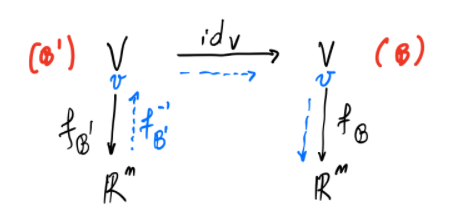
\includegraphics[scale=0.5]{cambiamento_di_base}
\end{center}
\[id_V: V\rightarrow V\]
\[v\mapsto v=id_V(v)\]
($id_V$ è una trasformazione lineare biunivoca) è l'elemento neutro nella composizione delle trasf.lineari da $V$ in se.

\textbf{Richiamo} Se $\mathcal{B}$ è una base, allora l'applicazione
\[f_{\mathcal{B}}: V\rightarrow \mathbb{R}\]
\[v\rightarrow \begin{bmatrix}x_1\\\vdots\\x_n\end{bmatrix}\]
Se $v=x_1v_1+...+x_nv_n$, $\begin{bmatrix}x_1\\\vdots\\x_n\end{bmatrix}=f_{\mathcal{B}}(v)$ è:
\begin{itemize}
  \item Lineare
  \item Biunivoca
\end{itemize}

\begin{center}
  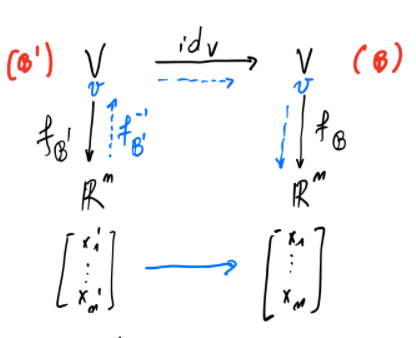
\includegraphics[scale=0.5]{cambiamento_base_2}
\end{center}
\[v=x'_1v'_1+x'_2v'_2+x'_3v'_3=f_{\mathcal{B}'}^{-1}\begin{bmatrix}x_1\\x_2\\x_3\end{bmatrix}\]
\[f_{\mathcal{B}}\circ id_V\circ f_{\mathcal{B}'}^{-1}\]
Siano:

$f_{\mathcal{B}}(v)=\begin{bmatrix}x_1\\\vdots\\x_n\end{bmatrix}$ le coordinate di $v$ in base $\mathcal{B}$

$f_{\mathcal{B}'}(v)=\begin{bmatrix}x'_1\\\vdots\\x'_n\end{bmatrix}$ le coordinate di $v$ in base $\mathcal{B}'$

Allora esiste un'unica applicazione $\Psi$ che rende il diagramma commutativo:
\[\Psi=f_{\mathcal{B}}\circ id_V \circ f_{\mathcal{B}'}^{-1}\]
ed esiste un'unica matrice $B$ tale che:
\begin{itemize}
\item \[f_{\mathcal{B}}=L_B \circ f_{\mathcal{B}'}\]
  \[=L_B\circ f_{\mathcal{B}'}(v) (\in\mathbb{R})\]
  \[L_B(f_{\mathcal{B}'}(v))=B\begin{bmatrix}x_1\\\vdots\\x_n\end{bmatrix}\]
  (con $L_B$ la trasformazione lineare associata alla moltiplicazione per $B$:
  \[L_B: \mathbb{R}^n\rightarrow\mathbb{R}^n\]
  \[Y\mapsto L_B(Y)=BY\]
  \[Y\mapsto Y)\]

\item Se $X=f_{\mathcal{B}}(v)\;\;\;\;\;X'=f_{\mathcal{B}'}(v)$ allora:
  \[X=BX'\]\[\text{ \textbf{Trasformazione delle coordinate}}\]
  Se $\mathcal{B}$ è la base vecchia e $\mathcal{B}'$ è la base nuova, allora le coordinate di un vettor $v$ nella base nuova si esprimono come:
  \[X'=B^{-1}X\]
  \\(\textit{Oss.}: $\Psi(X')=X, \Psi=L_B$ per un'opportuna matrice $B$.)

\item $B$ si chiama la matrice del cambiamento di base e si ottiene come:
  $B_{n\times n}[y_1\dots y_n]$, dove $y_i=\begin{bmatrix}\\ \\ \\\end{bmatrix}$ sono le coordinate di $v_i$ nella base $B$.
  \\Cioè $B=[f_{\mathcal{B}}(v'_1),...,f_{\mathcal{B}}(v'_n)]$, cioè è la matrice che contiene come colonne consecutive le coordinate dei vettori della base nuova espressi nella base vecchia, ovvero:
  \[\mathcal{B}=\mathcal{B}'\cdot B\]

\subsection{Def: Matrice associata a una trasformazione lineare $T$}
(opp. matrice che rappresenta $T$ rispetto alle basi degli spazi vettoriali)
\\L'unica matrice che rende il diagramma commutativo (cioè tale che $f_C\circ T\circ f_{\mathcal{B}}^{-1}=L_A$) si chiama matrice associata a $T$ nelle basi $\mathcal{B}$ e $\mathcal{C}$.
\\In altre parole $f_{\mathcal{C}}\circ T= L_Af_{\mathcal{B}}$, ovvero $f_{\mathcal{C}}(T(v))= Af_{\mathcal{B}}(v)A$.
\\In altre parole:
\[\underline{x}=f_{\mathcal{B}}(v)\]
\[\underline{y}=f_{\mathcal{C}}T((v))\]
\[\Rightarrow \underline{y}=A\underline{x}\]

\subsection{Proposizione}
\begin{itemize}
\item $V$ ha due basi $\mathcal{B}$ e $\mathcal{B}'$, sia $B$ la matrice del cambio di base da $\mathcal{B}$ a $\mathcal{B}'$:
  \[\mathcal{B}'=\mathcal{B}B\]

\item $W$ ha due basi $\mathcal{C}$ e $\mathcal{C}'$, sia $C$ la matrice del cambio di base da $\mathcal{C}$ a $\mathcal{C}'$:
  \[\mathcal{C}'=\mathcal{C}C\]

\item Se $T:V\rightarrow W$ una trasformazione lineare, con
  \begin{itemize}
  \item $A$ è la matrice che rappresenta $T$ nelle basi $\mathcal{B}$ e $\mathcal{C}$.
  \item $A'$ è la matrice che rappresenta $T$ nelle basi $\mathcal{B}'$ e $\mathcal{C}'$.
  \end {itemize}
  
\end{itemize}

\begin{enumerate}

\item Allora $A'=B^{-1}AC$ (cambiamento di matrice che rappresenta $T$)
\item Nel caso in cui $W=V$, e se prendo la stessa base per $V$ (cioe $\mathcal{C}=\mathcal{B}$) e sia $\mathcal{B}'$ un'altra base di $V$.
\\Se $B$ è la matrice del cambiamento di base da $\mathcal{B}$ a $\mathcal{B}'$, la nuova mtrice che rappresenta $T$ nella base $\mathcal{B}'$ è data da:
  \[A'=B^{-1}AB\]
  cioè $A'$ è coniugata tramite la matrice $B$ del cambiamento di base.

\end{enumerate}
\end{itemize}

\subsection{Definizione: matrice simile}
Si dice che una matrice quadrata $A$ è simila ad una matrice $A'\Leftrightarrow\exists\; B$ invertibile tale che:
\[A'=B^{-1}AB\]

\subsection{Proposizione}
Data $T:V\rightarrow V$ (endomorfismo) sia $\mathcal{B}$ una base di $V$ e sia $A$ la matrice (quadrata) associata a $T$ nella base $\mathcal{B}$.
\begin{enumerate}
\item Se $\mathcal{B}'$ è un'altra base di $V$, allora la matrice $A'$ associata a $T$ nella base $\mathcal{B}$ è data da:
  \[A'=D^{-1}AD\]
  Cioè esiste $D$ $n\times n$ invertibile tale che $A'$ è coniugata di $A$ tramite $D$.
  \\Con $D$ invertibile e che rappresenta la matrice del cambiamento di base da $\mathcal{B}$ a $\mathcal{B}'$.

\item Se $A'$ è una matrice simile ad $A$, allora esiste una base $\mathcal{B}'$ di $V$ tale che $A'$ è la matrice che rappresenta $T$ in base $\mathcal{B}'$!

\end{enumerate}

\subsection{Proposizione}
La relazione tra matrici $n\times n$ definita da:
\[A\sim B\Leftrightarrow\exists C\text{ invertibile con } B=C^{-1}AC\]
è una relazione di equivalenza su $\mathcal{M}_n(\mathbb{R})$
\textbf{R)}: $\forall A\in\mathcal{M}_n(\mathbb{R}):\;A\sim A$?
\\Cerco $C:\; A=C^{-1}AC$. Basta prendere $C=I_n$:
\[A=I^{-1}_nAI_n\;\;\;(I_n^{-1}=I_n)\]
\\\\\textbf{S)}: $\forall A,B\in\mathcal{M}_n(\mathbb{R}):\;\;A\sim B\Rightarrow B\sim A$?
\\Se $A\sim B$ allora $\exists C$ (invertibile) con $B=C^{-1}AC$. Ora devo ricavare $A$ da qui moltiplicando a sinistra per $C$ e destra per $C^{-1}$:
\[CBC^{-1}=CC^{-1}ACC^{-1}=A\]
Cioè $B\sim A$ (tramite $C^{-1}$): $A=(C^{-1})^{-1}BC^{-1}$.
\\\\\textbf{T)} $\forall A,B,C:\; A\sim B$ e $B\sim C\Rightarrow A\sim C$
\begin{itemize}

\item $\exists H:\;\; B=H^{-1}AH$

\item $\exists K:\; C=K^{-1}BK$

\end{itemize}

\[\Rightarrow C=K^{-1}BH=K^{-1}(H^{-1}AH)K=\]
\[=(K^{-1}H^{-1})A(HK)\]
\[=(HK)^{-1}A(HK)\]
\[=S^{-1}AS\;\;(HK=S)\]

\subsection{$\mathcal{M}_n(\mathbb{R})_{/\sim}$ Quoziente modulo la similitudine}
La classe di similitudine di una matrice $A\in \mathcal{M}_n(\mathbb{R})$, denotata con $\mathcal{O}_A$:
\[\mathcal{O}_A:=\{B\in\mathcal{M}_n(\mathbb{R}): A\sim B\}=\{B:\exists C, B=C^{-1}AC\}\]
è l'insieme delle matrici simili ad $A$.

A ogni endomorfismo di $T:V\rightarrow V$ si può associare in modo unico una classe di similitudine (che contiene tutte e sole le matrici che rappresentano $T$ nelle diverse basi).

\subsection{Definizioni: autovettore, autovalore, spettro di $T$, autospazio}
Sia $T:V\rightarrow V$ (endomorfismo) e sia $v\neq\underline{0}_V$:
\begin{itemize}
\item $v$ è un \textbf{autovettore} per $T$ se esiste $\lambda\in\mathbb{R}$ scalare tale che:
  \[T(v)=\lambda v\]
\item Tale $\lambda$ si chiama \textbf{autovalore} relativo all'autovettore $v$ (associato all'autovettore $v$)
\item L'insieme di tutti gli autovalori (se esistono) di una trasformazione $T$ si chiama \textbf{spettro di $T$}
  \[Spec(T)=\{\lambda\in K:\exists v\neq 0, v\in V\text{ con } T(v)=\lambda v\}\]

\item Si chiama \textbf{autospazio} relativo a un autovalore di $\lambda$ di $T$ il sottospazio $V_\lambda \leq V$ definito da:
  \[V_\lambda=\{v\in V:T(v)=\lambda v\}\]

\end{itemize}

\subsection{Osservazione}
Vedremo che lo spettro di $T$ non dipende dalla matrice che rappresenta $T$ in una base, cioè è una nozione intrinseca: se $A,B$ sono due matrici che rappresentanto $T$ in due basi diverse (cioè sono simili), allora $Spec(A)=Spec(B)$ dove $Spec(A)=Spec(L_A)$.
\begin{itemize}
\item $Spec(T)$ (o di una matrice) può essere vuoto.
\item Sia $\lambda_0$ un autovalore di $T$:
  \[V_{\lambda_0}=\{v\in V: T(v)=\lambda_0 V\}\]
  \[=\{v\in V: T(v)-\lambda_0id(v)=0\}\]
  \[=\{v\in V:(T-\lambda_0I)(v)=0\}\]
  \[=Ker(T-\lambda_0I)\neq\{0_V\}\]
\end{itemize}

\subsection{Proposizione}
\begin{enumerate}
\item $\lambda$ è un autovalore per $T\Leftrightarrow T-\lambda id_V$ è una trasformazione singolare (una trasformazione lineare è singolare se ha nucleo non vuoto).
\item Se $v$ è autovettore relativo a $\lambda$, allora non può essere autovettore relativo a un altro scalare $\mu\neq\lambda $, infatti:
  \[Av=\lambda V\text{ e anche } Av=\mu v\]
  \[\Rightarrow \lambda v=\mu v \Leftrightarrow \lambda v-\mu v=0_V\]
  \[(\lambda -\mu)v=0_V\]
  che è una contraddizione perchè $v\neq 0$ perchè autovettore e $\lambda-\mu\neq 0$.

  \item Autovettori relativi ad autovalori distinti sono linearmente indipendenti.

\end{enumerate}

\subsection{Diagonalizzazione di una matrice}
\begin{itemize}
\item Un endomorfismo $T:V\rightarrow V$ di $V$ è diagonalizabile $\Leftrightarrow$ esiste una base di $T$ fatta di autovettori.
  \\$\Rightarrow$ in base $\mathcal{B}$ la matrice che rappresenta $T$ è diagonale.

\item Ogni matrice che rappresenta $T$ in qualche base ha gli stessi autovalori di $T$, cioè:
  \[Spec(L_A)=Spec(A)=Spec(T)\]

\item L'autospazio relativo all'autovalore $lambda $,
  \[V_\lambda=\{v\in V: T(v)=\lambda v\}=Ker(T-\lambda id)\]

\item Autovettori relativi ad autovalori distinti sono indipendenti.

\item $\lambda$ autovalore di $T\Leftrightarrow T-\lambda id_V$ è singolare ($Ker(T-\lambda id_V)\neq\{0_V\}$).

\item Se $A$ è la matrice della trasformazione $L_A:\mathbb{R}^n\rightarrow\mathbb{R}^n$ (nella base canonica) $A$ ha un autovalore $\lambda\Leftrightarrow$ la matrice $(A-\lambda I_n)$ è singolare $\Leftrightarrow$ $Ker(A-\lambda I_n)$ è non banale $\Leftrightarrow det(A-\lambda I_n)=0$.
  
\end{itemize}

\subsection{Polinomio caratteristico}
Si chiama polinomio caratteristico di $T:V\rightarrow V$ il polinomio:
\[p_T(\lambda)=det(T-\lambda id_V)\]

\subsection{Proposizione}
Se $A$ e $B$ sono simili, allora hanno lo stesso polinomio caratteristico: cioè se $A$ e $B$ rappresentano (in basi diverse) la stessa trasformazione $T$: allora
\[det(A-\lambda I_n)=det(B-\lambda I_n)\]
\textbf{Dimostrazione}: $A\sim B\Leftrightarrow \exists C$ invertibile con $B=C^{-1}AC$.
\\Osserviamo che:
\[C^{-1}(A-\lambda I_n)C=\]
\[=(C^{-1}A-C^{-1}\lambda I_n)C\]
\[=C^{-1}AC-C^{-1}\lambda I_nC\]
\[=B-\lambda C^{-1}I_n C\]
\[=B-\lambda I_n\]

Infine:
\[det(B-\lambda I_n)=det(C^{-1}(A-\lambda I_n)C=\]
\[det(C^{-1})det(A-\lambda I_n)det(C)=\]
\[det(C^{-1})det(C)det(A-\lambda I_n)=\]
\[\frac{1}{det(C)}det(C)det(A-\lambda I_n)=\]
\[det(A-\lambda I_n)\]
Quindi possimao dire che $p_T(\lambda)=p_A(\lambda)$ per ogni matrice $A$ nella classe di similitudine.

\subsection{Proprietà del polinomio caratteristico}
\begin{itemize}

\item $p_T(\lambda)=det(A-\lambda I)$ ($A$ che rappresenta $T$ in una base)

\item $p_T(\lambda)$, $(p_A(\lambda))$ è un polinomio:
  \begin{itemize}
  \item di grado $n$ in $\lambda $
  \item Il coefficiente di $\lambda ^n$ è $(-1)^n$
  \item Il coefficiente di $\lambda^{n-1}$ è $(-1)^ntr(A)$ ($traccia(A)=$somma degli el. sulla diagonale)
  \item Il coefficiente di $\lambda ^0=1$ (del termine noto) è $(-1)^0detA=detA$
  \end{itemize}

\item $v\neq 0$ e $Av=\lambda v \Leftrightarrow$
  \[(A-\lambda I)v=0\;\;(v\neq 0)\]
  \[\Leftrightarrow (A-\lambda I)singolare\]
  \[\Leftrightarrow det(A-\lambda I)=0\;\;(p_T(\lambda))\]
  \[\Leftrightarrow\lambda\text{ è radice del polinomio caratteristico}\]

\end{itemize}

\subsection{Corollario}
Se $p_T(\lambda)$ ha $n$ soluzioni distinte, allora $T$ è diagonalizzabile.

\subsection{Def: molteplicità algebrica radice}
Si chiama \textbf{molteplicità algebrica} di una radice $x_0$ (soluzione) di un polinomio $p(x)$ un numero $k$ tale che $(x-x_0)^k|p(x)$ ma $(x-x_0)^{k+1}\nmid p(x)$
  \[p(x)=(x-x_0)^kq(x)\]

\subsection{Def: molteplicità algebrica $\lambda_0$}  
Si chiama \textbf{molteplicità algebrica} di $\lambda_0$ (autovalore di $T$) e si denota con $m_a(\lambda_0)$ la molteplicità algebrica di $\lambda_0$ come radice di $p_T(\lambda)$, cioè:
  \[p_T(\lambda)=(\lambda -\lambda_0)^{m_a(\lambda_0)}(\;\;\;)\]

\subsection{Def: molteplicità geometrica $\lambda_0$}
Si chiama \textit{molteplicità geometrica} di $\lambda_0$ (autovalore di $T$) e si indica con $m_g(\lambda_0)$, la dimensione dell'autospazio di $V_{\lambda_0}$ relativo a $\lambda_0$, cioè la nullità di $T-\lambda_0 I$.
  \\In genere $m_g(\lambda_0)\leq m_a(\lambda_0)$

\subsection{Teorema}
Le seguenti sono equivalenti per $T:V\rightarrow V, \; dim_KV=n$:
\begin{enumerate}
\item $T$ è diagonalizzabile $\Leftrightarrow $

\item $T$ ha tutti i suoi autovalori in $K$ (cioè il polinomio caratteristico si spezza in fattori del tipo $(x-a)^*$ lineari di grado 1) e la molteplicità algebrica di ogni autovalore coincide con la molteplicità geometrica:
  \[m_a(\lambda_0)=m_g(\lambda_0)\;\;\forall\lambda_0\in Spec(T)\]
  quindi se con $Spec(T)=\{\lambda_1,...,\lambda_k\}$ allora $n=m_g(\lambda_1)+...+m_g(\lambda_k)$.

\end{enumerate}
